Closed loop simulations, with the control logic of the zigzag test, were used to predict the model test experiments. Comparisons of these predictions are shown in \autoref{fig:closed_loop_zigzag10} and \autoref{fig:closed_loop_zigzag20}. The drift angle $\beta$, heading angle $\psi$, and yaw rate $r$, are in good agreement with the experiments for all the models, especially the heading -- which is the most important quantity in zigzag tests; The mathematical model does however have a faster response time.
\begin{figure}[h]
    \centering
    \includesvg[width=\columnwidth]{figures/results.closed_loop_zigzag10.svg}
    \caption{Results from a zigzag10/10 model test compared with closed loop simulations.}
    \label{fig:closed_loop_zigzag10}
\end{figure}
\begin{figure}[h]
    \centering
    \includesvg[width=\columnwidth]{figures/results.closed_loop_zigzag20.svg}
    \caption{Results from a zigzag20/20 model test compared with closed loop simulations.}
    \label{fig:closed_loop_zigzag20}
\end{figure}

An alternative comparison, is to compare model predictions with inverse dynamics forces from the model tests; This comparison gives more detailed information about the forces and moments involved during the manoeuvres. The models predicts the forces and moments for the estimated state of the experiment. Thus, all models predict the same state in contrast to simulations -- where the states may differ as the solutions begin to deviate. Inverse dynamics comparisons are shown in \autoref{fig:ID_zigzag10} for the zigzag10/10, and in \autoref{fig:ID_zigzag20} for the zigzag20/20.    
It seems that the total yawing moments $N_D$ agree well for all models and the experimental data. For the total sway force $Y_R$ the mathematical model seem to predict a little bit higher force.  
It can also be seen that the Reference model and PISM predicts the exact same rudder yawing moment $N_R$, since they both use the same deterministic semi-empirical rudder model -- the yawing moments from the hull $N_H$ are therefore similar for these models. The rudder yawing moment from the mathematical model is however very different; The regression has thus been forced to also make the yawing moments from the hull $N_H$ to be very different -- so that the total yawing moment adds up to be correct. This means that the total yawing moment is the same for all models, but the decomposition of hull and rudder moments turns out to be very different.
\begin{figure}[h]
    \centering
    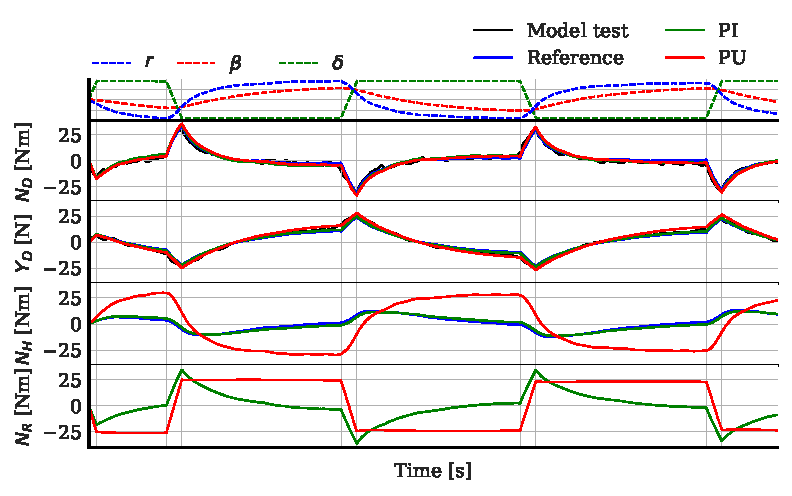
\includegraphics[width=\columnwidth]{figures/results.ID_zigzag10.pdf}
    \caption{Inverse dynamics estimations of $Y_D$, and $N_D$ during a zigzag10/10 model test compared with model predictions.}
    \label{fig:ID_zigzag10}
\end{figure}
\begin{figure}[h]
    \centering
    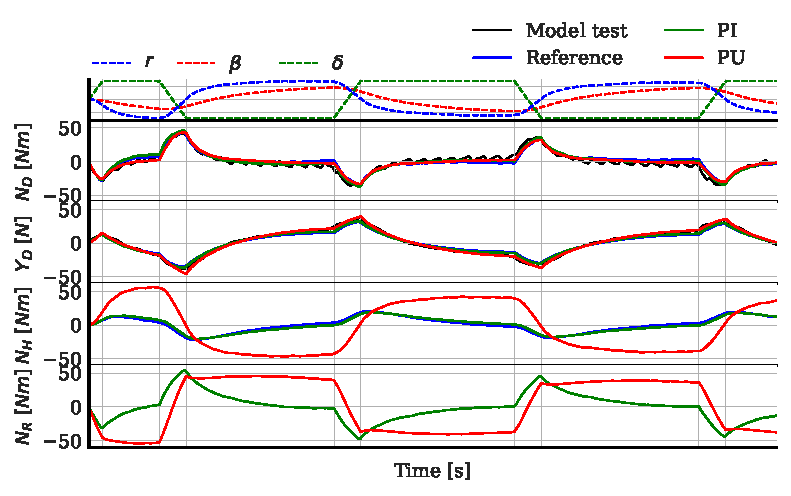
\includegraphics[width=\columnwidth]{figures/results.ID_zigzag20.pdf}
    \caption{Inverse dynamics estimations of $Y_D$, and $N_D$ during a zigzag20/20 model test compared with model predictions.}
    \label{fig:ID_zigzag20}
\end{figure}

The hull force model can be closer examined by decomposing the individual parameter contributions. \autoref{fig:ID_regression_N_decomposition} shows the parameter decomposition for the two models together with the Reference model. The graphs show the joined contributions for parameters related to drift, and yaw rate. It seems that PISM and the Reference model have very similar parameter decompositions.
The parameter decomposition of the mathematical model is completely different, where almost the entire contribution to the hull yawing moment $N_H$ can be denoted to the yaw rate parameters; The sway force due to drift is also very large.  
\begin{figure}[h]
    \begin{center}
        \includesvg[width=\columnwidth]{figures/results.hull_force_decomposition_zigzag20.svg}
        \caption{Decomposition of hull forces and moments during a zigzag20/20 test for parameters related to drift, yaw rate the prediction models.}
        \label{fig:ID_regression_N_decomposition}
    \end{center}
\end{figure}
Possible implications of that the mathematical model have this physically incorrect decomposition of the hull's drift angle and yaw rate dependence will be further investigated in the next section.